
\documentclass[border=10pt, 12pt]{standalone}
\usepackage[svgnames]{xcolor}
\usepackage{amsmath}
\usepackage{pgfplots}
\pgfplotsset{compat=newest}
\usepackage[sfdefault]{FiraSans}
\usepackage{FiraMono}
\renewcommand*\familydefault{\sfdefault}
\begin{document}
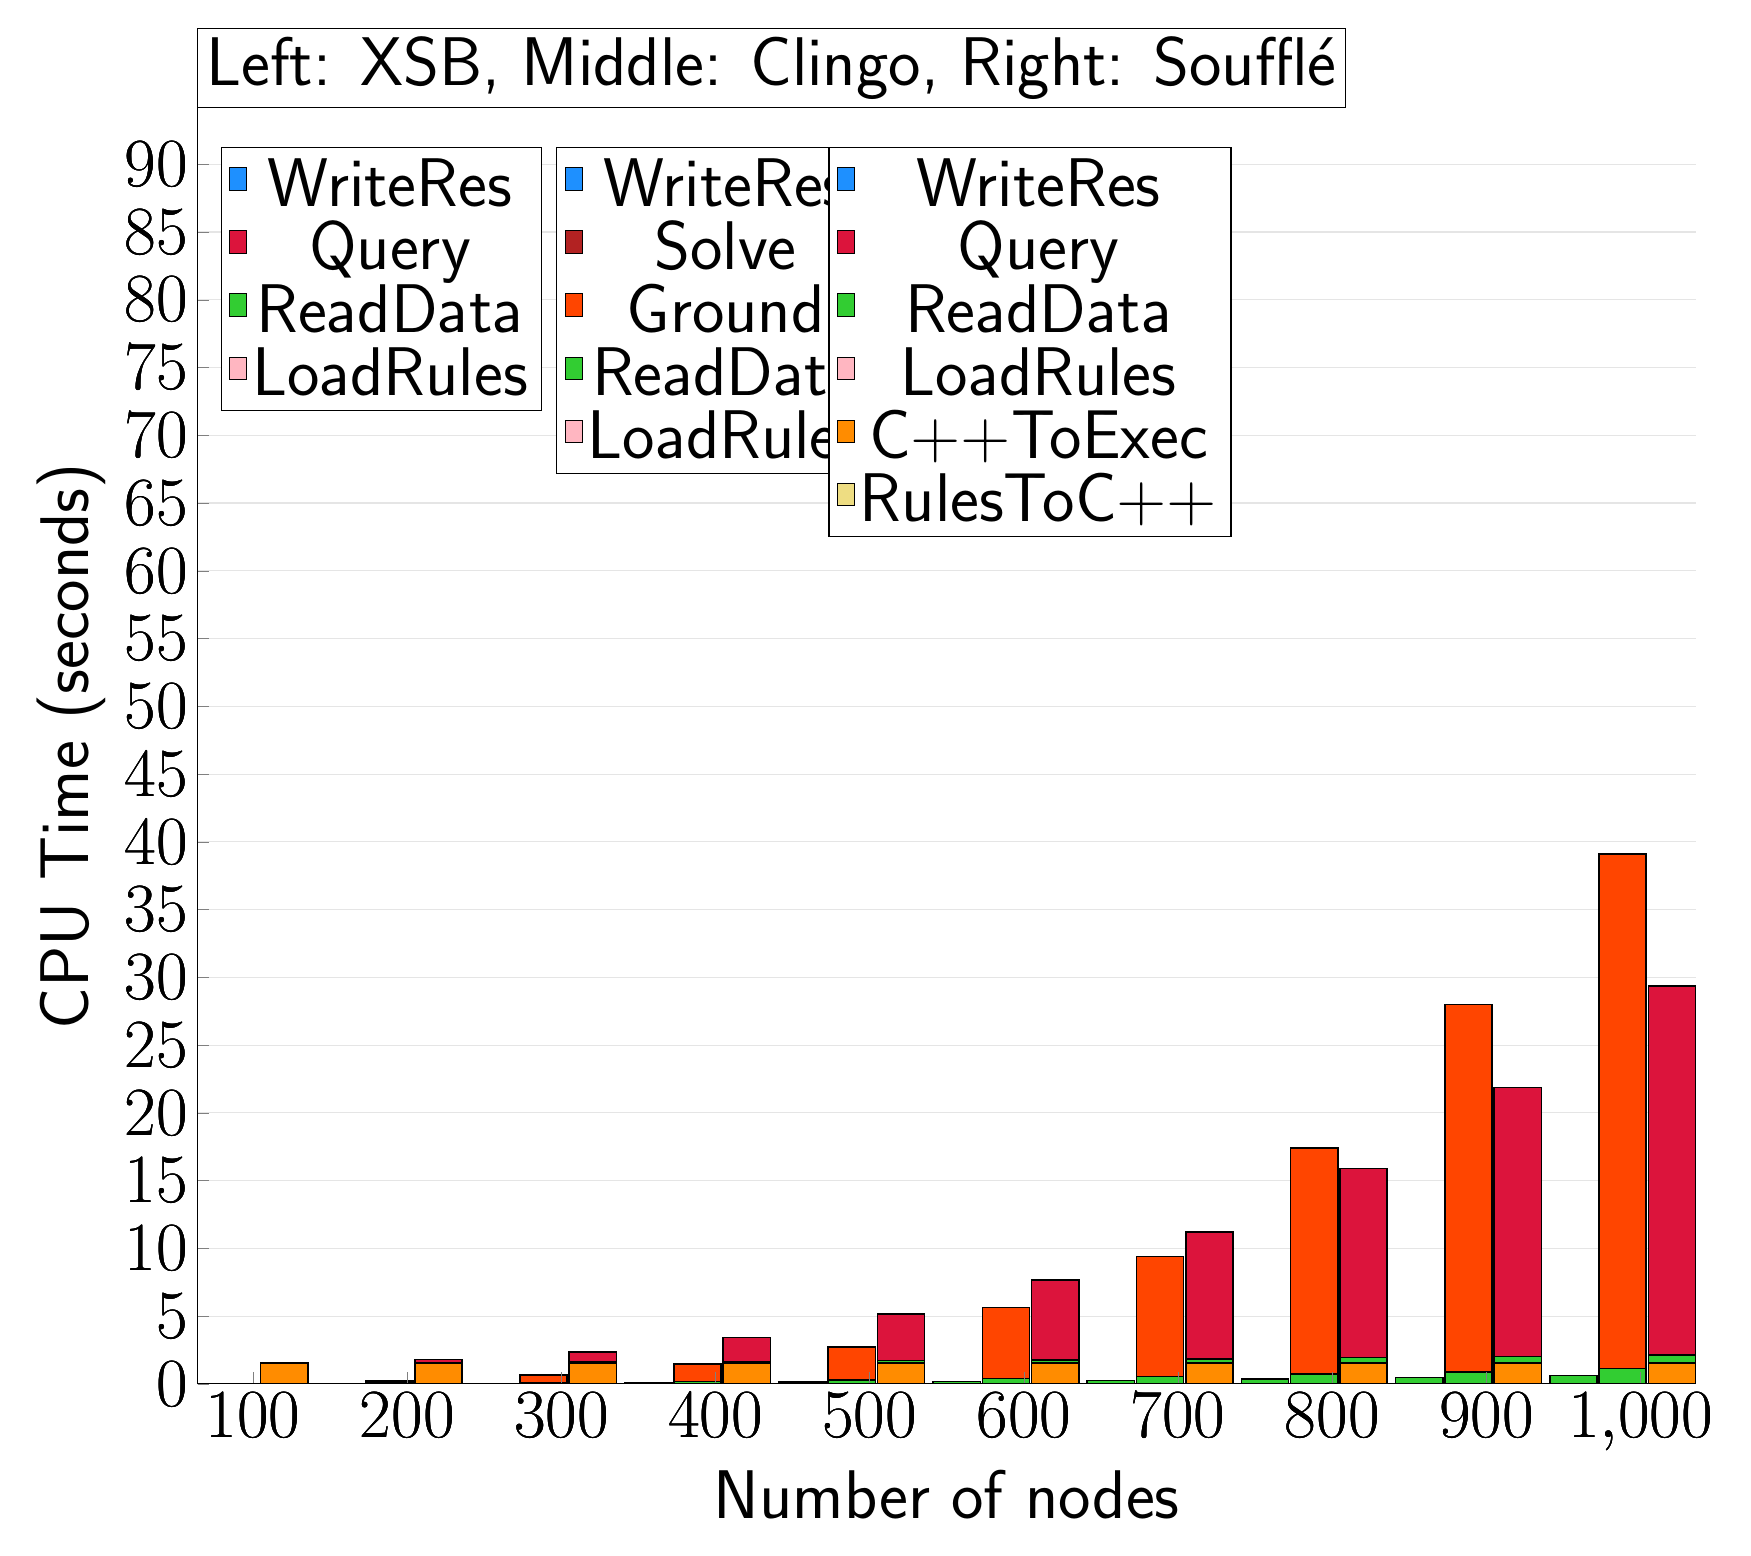
\begin{tikzpicture}
                        \begin{axis}[bar shift=-24.3pt, 
   ybar stacked,
   width=1.7\textwidth,
   bar width=0.6cm,
   ymajorgrids, tick align=inside,
   major grid style={draw=gray!20},
   xtick=data,
   ymin=0, ymax=94.12288,
   axis x line*=bottom,
   axis y line*=left,
   enlarge x limits=0.04,
   legend style={
       at={(0.23, 0.97)},
       anchor=north east,
       legend columns=1,
       font=\Huge,
   },
   ylabel={CPU Time (seconds)},
   xlabel={Number of nodes},
   label style={font=\Huge},
   tick label style={font=\Huge},
]
\addlegendimage{fill=DodgerBlue, draw=black, line width=0.2pt}
\addlegendentry{WriteRes}
\addlegendimage{fill=Crimson, draw=black, line width=0.2pt}
\addlegendentry{Query}
\addlegendimage{fill=LimeGreen, draw=black, line width=0.2pt}
\addlegendentry{ReadData}
\addlegendimage{fill=LightPink, draw=black, line width=0.2pt}
\addlegendentry{LoadRules}
\addplot +[fill=LightPink, draw=black, line width=0.55pt] coordinates {
(100, 0.000554)
(200, 0.0005514000000000004)
(300, 0.0005573999999999999)
(400, 0.0005534000000000002)
(500, 0.0005605999999999999)
(600, 0.0005496000000000002)
(700, 0.0005518000000000001)
(800, 0.0005555999999999998)
(900, 0.0005539999999999996)
(1000, 0.0005546000000000004)
};
\addplot +[fill=LimeGreen, draw=black, line width=0.55pt] coordinates {
(100, 0.004037000000000001)
(200, 0.017065399999999998)
(300, 0.040211399999999994)
(400, 0.074549)
(500, 0.122703)
(600, 0.18309920000000002)
(700, 0.2594006)
(800, 0.3534384)
(900, 0.4685638)
(1000, 0.6077686)
};
\addplot +[fill=Crimson, draw=black, line width=0.55pt] coordinates {
(100, 2.800000000000024e-06)
(200, 3.000000000000224e-06)
(300, 4.400000000001623e-06)
(400, 5.5999999999972715e-06)
(500, 6.000000000000448e-06)
(600, 5.6000000000055995e-06)
(700, 5.3999999999776425e-06)
(800, 6.20000000000065e-06)
(900, 5.8000000000113515e-06)
(1000, 6.199999999978446e-06)
};
\addplot +[fill=DodgerBlue, draw=black, line width=0.55pt] coordinates {
(100, 5.9999999999999656e-05)
(200, 6.239999999999928e-05)
(300, 6.139999999999897e-05)
(400, 6.400000000000294e-05)
(500, 6.320000000000769e-05)
(600, 6.819999999999045e-05)
(700, 6.300000000000194e-05)
(800, 6.600000000001048e-05)
(900, 6.960000000000298e-05)
(1000, 6.460000000005907e-05)
};
\end{axis}

\begin{axis}[bar shift=-6.5pt, 
   ybar stacked,
   width=1.7\textwidth,
   bar width=0.6cm,
   ymajorgrids, tick align=inside,
   major grid style={draw=none},
   xtick=data,
   ymin=0, ymax=94.12288,
   axis x line*=none,
   axis y line*=none,
   enlarge x limits=0.04,
   legend style={
       at={(0.454, 0.97)},
       anchor=north east,
       legend columns=1,
       font=\Huge,
   },
   label style={font=\Huge},
   tick label style={font=\Huge},
]
\addlegendimage{fill=DodgerBlue, draw=black, line width=0.2pt}
\addlegendentry{WriteRes}
\addlegendimage{fill=FireBrick, draw=black, line width=0.2pt}
\addlegendentry{Solve}
\addlegendimage{fill=OrangeRed, draw=black, line width=0.2pt}
\addlegendentry{Ground}
\addlegendimage{fill=LimeGreen, draw=black, line width=0.2pt}
\addlegendentry{ReadData}
\addlegendimage{fill=LightPink, draw=black, line width=0.2pt}
\addlegendentry{LoadRules}
\addplot +[fill=LightPink, draw=black, line width=0.55pt] coordinates {
(100, 0.0)
(200, 0.0)
(300, 0.0)
(400, 0.0)
(500, 0.0)
(600, 0.0)
(700, 0.0)
(800, 0.0)
(900, 0.0)
(1000, 0.0)
};
\addplot +[fill=LimeGreen, draw=black, line width=0.55pt] coordinates {
(100, 0.010000000000000009)
(200, 0.042000000000000016)
(300, 0.10000000000000005)
(400, 0.176)
(500, 0.272)
(600, 0.4040000000000001)
(700, 0.542)
(800, 0.722)
(900, 0.892)
(1000, 1.1280000000000001)
};
\addplot +[fill=OrangeRed, draw=black, line width=0.55pt] coordinates {
(100, 0.020000000000000018)
(200, 0.15599999999999997)
(300, 0.5360000000000001)
(400, 1.27)
(500, 2.432)
(600, 5.220000000000001)
(700, 8.868)
(800, 16.666)
(900, 27.086000000000002)
(1000, 37.96600000000001)
};
\addplot +[fill=FireBrick, draw=black, line width=0.55pt] coordinates {
(100, 0.0)
(200, 0.0)
(300, 0.0020000000000000018)
(400, 0.0)
(500, 0.002000000000000046)
(600, 0.005999999999999872)
(700, 0.00400000000000027)
(800, 0.003999999999999915)
(900, 0.003999999999999204)
(1000, 0.003999999999999204)
};
\addplot +[fill=DodgerBlue, draw=black, line width=0.55pt] coordinates {
(100, 0.0)
(200, 0.0020000000000000018)
(300, -0.0020000000000000018)
(400, 0.0020000000000000018)
(500, -0.002000000000000046)
(600, -0.005999999999999872)
(700, -0.00400000000000027)
(800, -0.003999999999999915)
(900, -0.003999999999999204)
(1000, -0.003999999999999204)
};
\end{axis}

\begin{axis}[bar shift=11.3pt, 
   ybar stacked,
   width=1.7\textwidth,
   bar width=0.6cm,
   ymajorgrids, tick align=inside,
   major grid style={draw=none},
   xtick=data,
   ymin=0, ymax=94.12288,
   axis x line*=none,
   axis y line*=none,
   enlarge x limits=0.04,
   legend style={
       at={(0.69, 0.97)},
       anchor=north east,
       legend columns=1,
       font=\Huge,
   },
   label style={font=\Huge},
   tick label style={font=\Huge},
]
\addlegendimage{fill=DodgerBlue, draw=black, line width=0.2pt}
\addlegendentry{WriteRes}
\addlegendimage{fill=Crimson, draw=black, line width=0.2pt}
\addlegendentry{Query}
\addlegendimage{fill=LimeGreen, draw=black, line width=0.2pt}
\addlegendentry{ReadData}
\addlegendimage{fill=LightPink, draw=black, line width=0.2pt}
\addlegendentry{LoadRules}
\addlegendimage{fill=DarkOrange, draw=black, line width=0.2pt}
\addlegendentry{C++ToExec}
\addlegendimage{fill=LightGoldenrod, draw=black, line width=0.2pt}
\addlegendentry{RulesToC++}
\addplot +[fill=LightGoldenrod, draw=black, line width=0.55pt] coordinates {
(100, 0.004000000000000001)
(200, 0.006000000000000001)
(300, 0.006000000000000001)
(400, 0.006000000000000001)
(500, 0.006000000000000001)
(600, 0.006000000000000001)
(700, 0.006000000000000001)
(800, 0.004000000000000001)
(900, 0.004000000000000001)
(1000, 0.007999999999999997)
};
\addplot +[fill=DarkOrange, draw=black, line width=0.55pt] coordinates {
(100, 1.52)
(200, 1.5299999999999998)
(300, 1.5240000000000002)
(400, 1.538)
(500, 1.534)
(600, 1.52)
(700, 1.53)
(800, 1.5340000000000003)
(900, 1.54)
(1000, 1.528)
};
\addplot +[fill=LightPink, draw=black, line width=0.55pt] coordinates {
(100, 0.00014359999999999997)
(200, 0.00013220000000000001)
(300, 0.00015180000000000003)
(400, 0.0001564)
(500, 0.00014900000000000002)
(600, 0.00015759999999999998)
(700, 0.0001502)
(800, 0.0001544)
(900, 0.00014820000000000002)
(1000, 0.0001454)
};
\addplot +[fill=LimeGreen, draw=black, line width=0.55pt] coordinates {
(100, 0.0131724)
(200, 0.037712800000000005)
(300, 0.0712506)
(400, 0.1129278)
(500, 0.16474819999999998)
(600, 0.22774740000000002)
(700, 0.3007996)
(800, 0.389318)
(900, 0.4849848)
(1000, 0.5950692)
};
\addplot +[fill=Crimson, draw=black, line width=0.55pt] coordinates {
(100, 0.0417046)
(200, 0.23057660000000002)
(300, 0.7562285999999999)
(400, 1.7739319999999998)
(500, 3.4337299999999997)
(600, 5.917778)
(700, 9.375504)
(800, 13.96048)
(900, 19.834139999999998)
(1000, 27.241300000000003)
};
\addplot +[fill=DodgerBlue, draw=black, line width=0.55pt] coordinates {
(100, 4.7600000000000005e-05)
(200, 5.9000000000000004e-05)
(300, 0.00012800000000000002)
(400, 0.0001312)
(500, 0.00015739999999999998)
(600, 0.000148)
(700, 0.00017240000000000002)
(800, 0.00017559999999999999)
(900, 0.0001868)
(1000, 0.0001984)
};
\end{axis}


\node[anchor=south, draw, fill=white] at (rel axis cs:0.42,1) {\Huge Left: XSB, Middle: Clingo, Right: Soufflé};
\end{tikzpicture}
\end{document}
                    